\documentclass[a4paper, 12pt]{article}

%\usepackage[cmex10]{amsmath, mathtools}
\usepackage{amsmath,amssymb,amsbsy,amsfonts,amsthm}
\usepackage{multirow}
\usepackage{bm}
\usepackage{enumerate}
\usepackage{url}
\usepackage[ruled,vlined]{algorithm2e}
\usepackage{fancyvrb}
\usepackage{yfonts}
\usepackage{dsfont}
\usepackage{calc} %    For the \widthof macro
\usepackage{xparse} %  For \NewDocumentCommand
\usepackage{wrapfig}
\usepackage{tikz}
\usepackage{lipsum}
%\input{../tikz.conf}

\usepackage{graphicx}
\usepackage{subcaption}

\usetikzlibrary{bayesnet}


\usepackage[margin=0.25in]{geometry}


\title{Networks Properties Properties}

\begin{document}

\maketitle
\tableofcontents

\clearpage

\section{$M_e$}
\subsection{Dancer Dataset}
\clearpage

    \begin{figure*}
        \centering
        \begin{subfigure}[b]{0.475\textwidth}
            \centering
            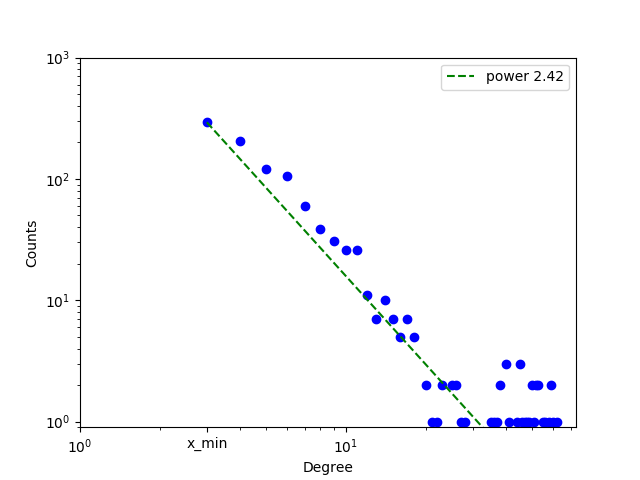
\includegraphics[width=\textwidth]{img/corpus/dancer_1/figure_1}
            \caption[Network2]%
            {{\small Network 1}}    
            \label{fig:mean and std of net14}
        \end{subfigure}
        \hfill
        \begin{subfigure}[b]{0.475\textwidth}  
            \centering 
            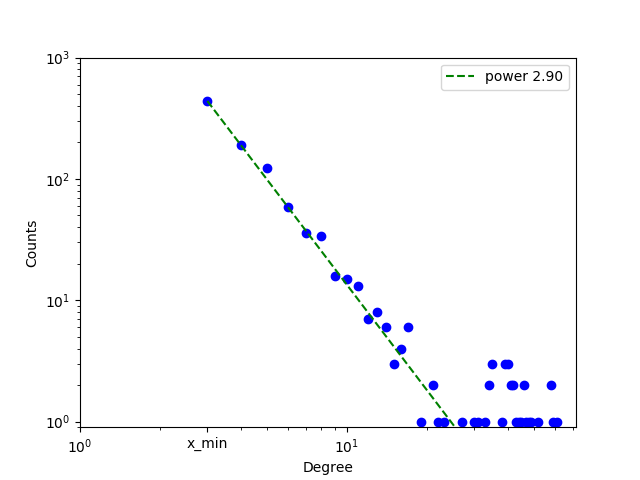
\includegraphics[width=\textwidth]{img/corpus/dancer_2/figure_1}
            \caption[]%
            {{\small Network 2}}    
            \label{fig:mean and std of net24}
        \end{subfigure}
        \vskip\baselineskip
        \begin{subfigure}[b]{0.475\textwidth}   
            \centering 
            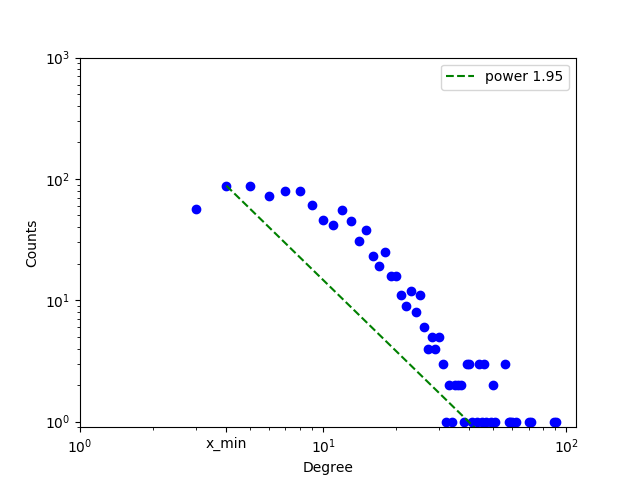
\includegraphics[width=\textwidth]{img/corpus/dancer_3/figure_1}
            \caption[]%
            {{\small Network 3}}    
            \label{fig:mean and std of net34}
        \end{subfigure}
        \quad
        \begin{subfigure}[b]{0.475\textwidth}   
            \centering 
            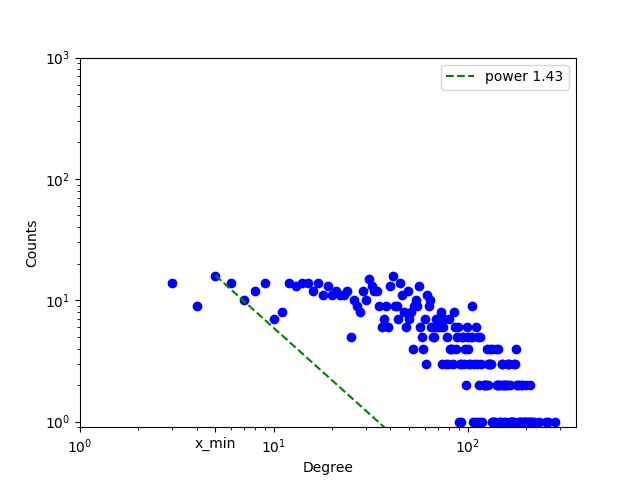
\includegraphics[width=\textwidth]{img/corpus/dancer_4/figure_1}
            \caption[]%
            {{\small Network 4}}    
            \label{fig:mean and std of net44}
        \end{subfigure}
        \caption[ The average and standard deviation of critical parameters ]
        {\small Global degree distribution in Dancer Synthetic Dataset.} 
        \label{fig:mean and std of nets}
    \end{figure*}

    \begin{table}
        \begin{tabular}{lrrrr}
            \hline
                       &   pvalue &   alpha &   x\_min &   n\_tail \\
                       \hline
                        Network 4 &    0.000 &   1.435 &       5 &  977.000 \\
                         Network 3 &    1.000 &   1.952 &       4 &  943.000 \\
                          Network 2 &    0.982 &   2.897 &       3 & 1000.000 \\
                           Network 1 &    1.000 &   2.424 &       3 & 1000.000 \\
                           \hline
        \end{tabular}

        \caption{Goodness of fit result fo the global degree distribution}
    \end{table}


    \begin{figure*}
        \centering
        \begin{subfigure}[b]{0.475\textwidth}
            \centering
            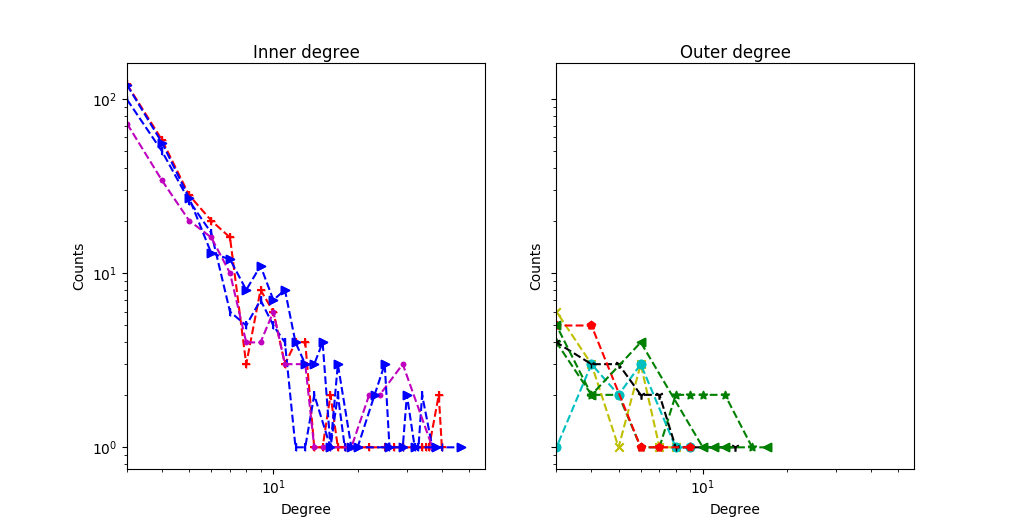
\includegraphics[width=\textwidth]{img/corpus/dancer_1/figure_2}
            \caption[Network2]%
            {{\small Network 1}}    
            \label{fig:mean and std of net14}
        \end{subfigure}
        \hfill
        \begin{subfigure}[b]{0.475\textwidth}  
            \centering 
            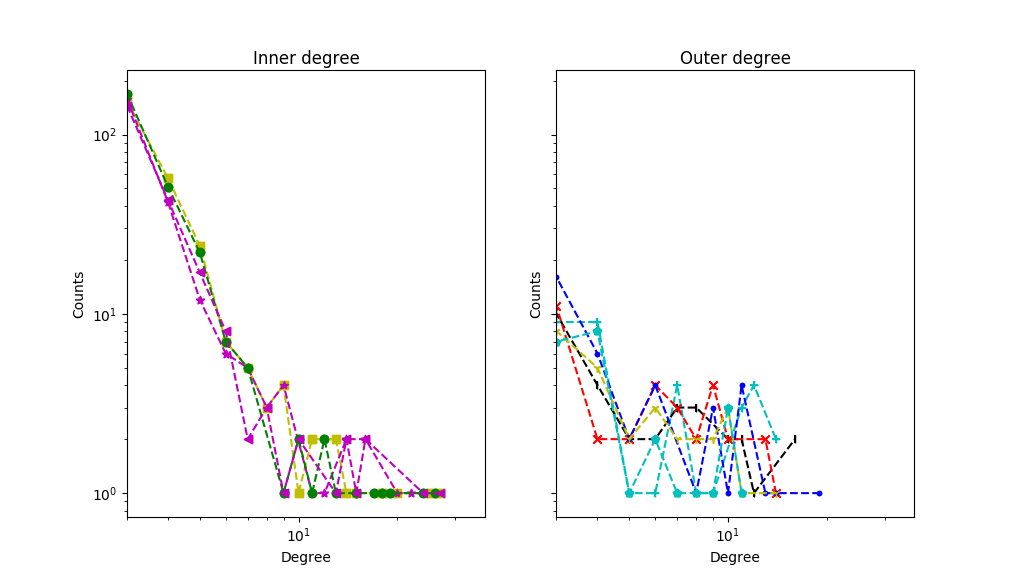
\includegraphics[width=\textwidth]{img/corpus/dancer_2/figure_2}
            \caption[]%
            {{\small Network 2}}    
            \label{fig:mean and std of net24}
        \end{subfigure}
        \vskip\baselineskip
        \begin{subfigure}[b]{0.475\textwidth}   
            \centering 
            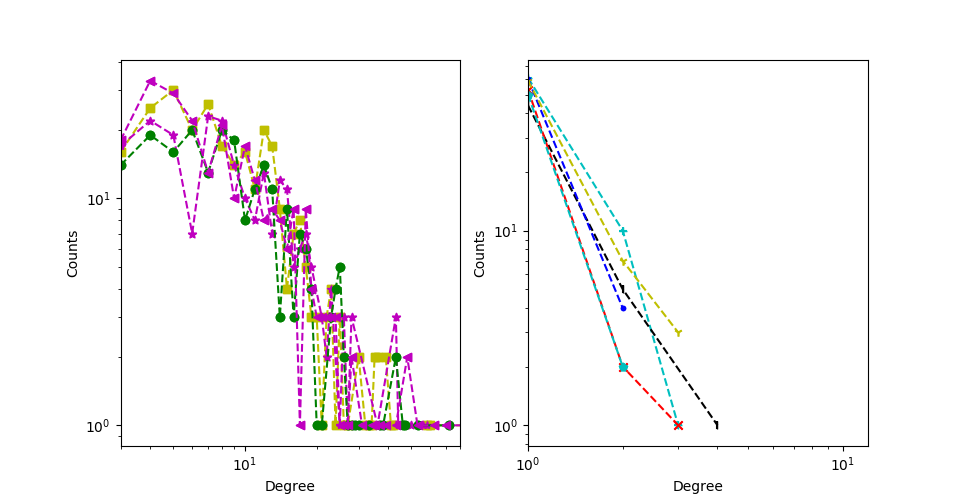
\includegraphics[width=\textwidth]{img/corpus/dancer_3/figure_2}
            \caption[]%
            {{\small Network 3}}    
            \label{fig:mean and std of net34}
        \end{subfigure}
        \quad
        \begin{subfigure}[b]{0.475\textwidth}   
            \centering 
            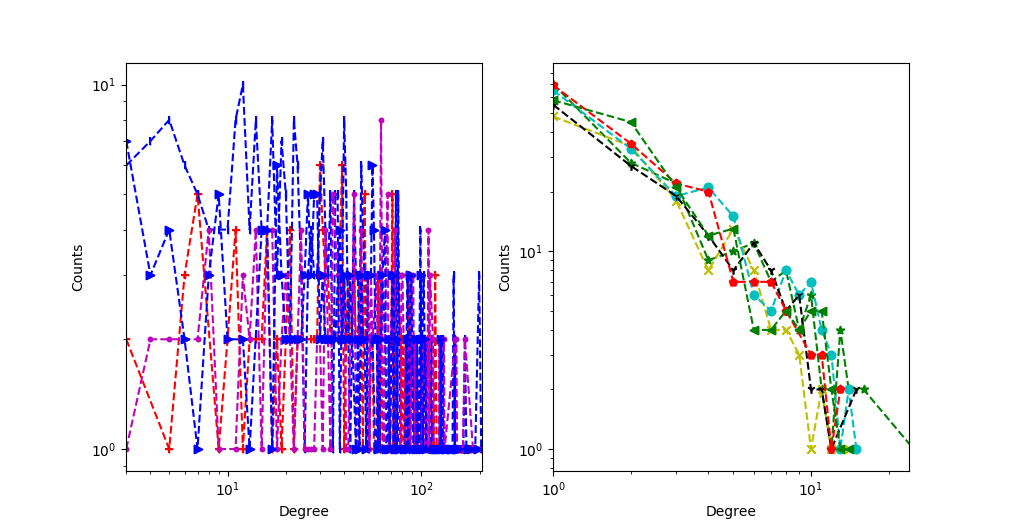
\includegraphics[width=\textwidth]{img/corpus/dancer_4/figure_2}
            \caption[]%
            {{\small Network 4}}    
            \label{fig:mean and std of net44}
        \end{subfigure}
        \caption[ The average and standard deviation of critical parameters ]
        {\small Local degree distribution. Inner and outer degree are seperated.} 
        \label{fig:mean and std of nets}
    \end{figure*}

\subsection{Burstiness}
\clearpage

\begin{figure}[ht]
    \vspace{-3cm}
	\centering IMMSB\\
	\minipage{0.27\textwidth}
	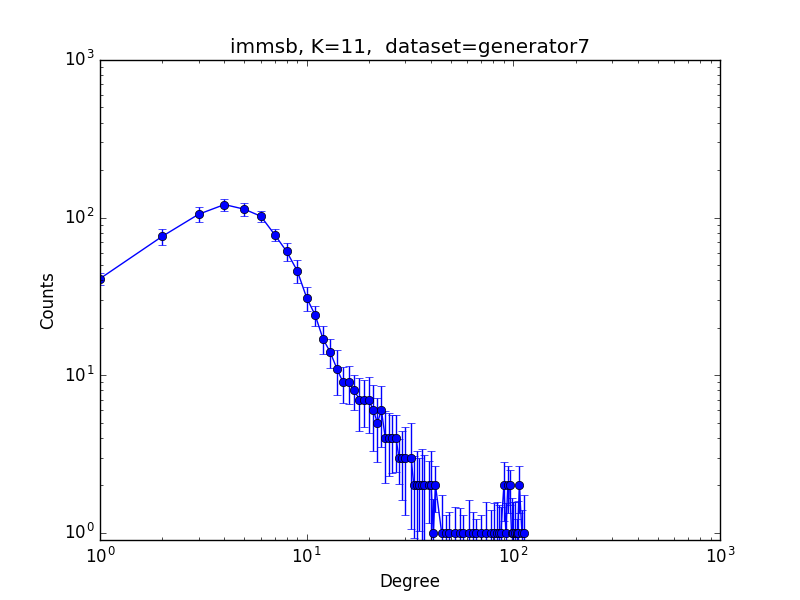
\includegraphics[scale=0.27]{img/expe/1_mmsb/figure_1}
	\endminipage
		\minipage{0.27\textwidth}
	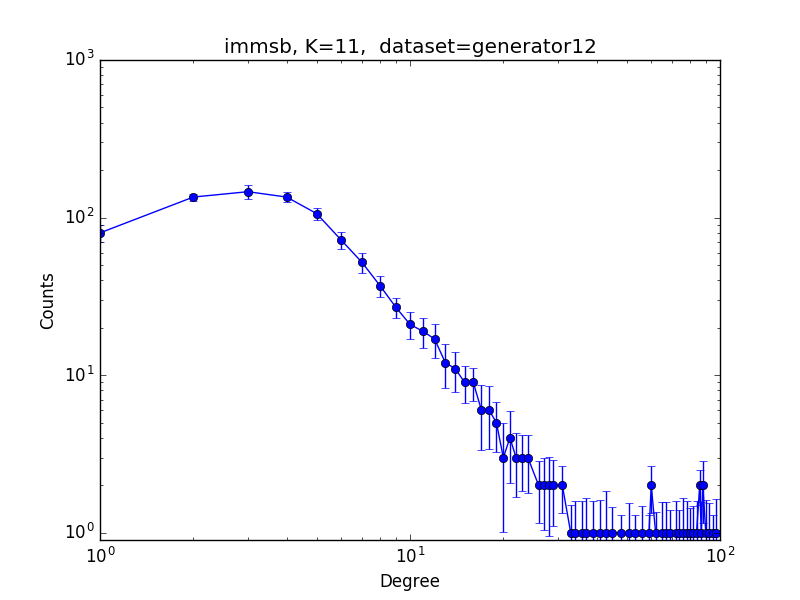
\includegraphics[scale=0.27]{img/expe/2_mmsb/figure_1}
	\endminipage
	\minipage{0.27\textwidth}
	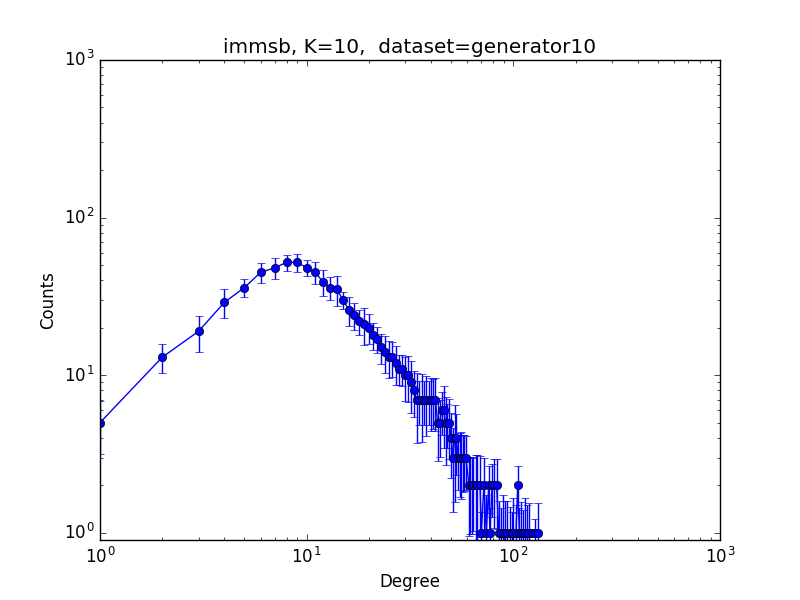
\includegraphics[scale=0.27]{img/expe/3_mmsb/figure_1}
	\endminipage
		\vspace{-0.29cm}
	\minipage{0.27\textwidth}
	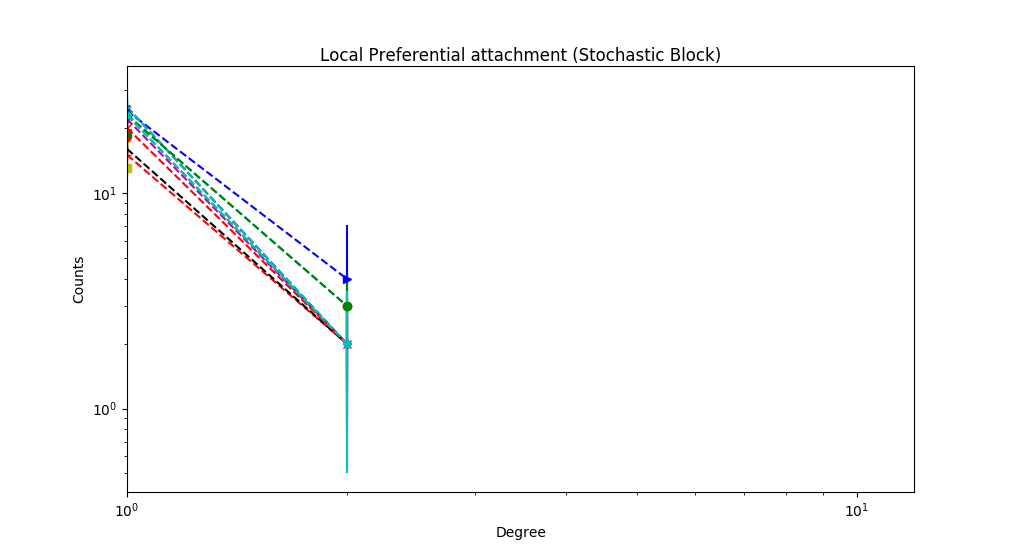
\includegraphics[scale=0.27]{img/expe/1_mmsb/figure_2}
	\endminipage
		\minipage{0.27\textwidth}
	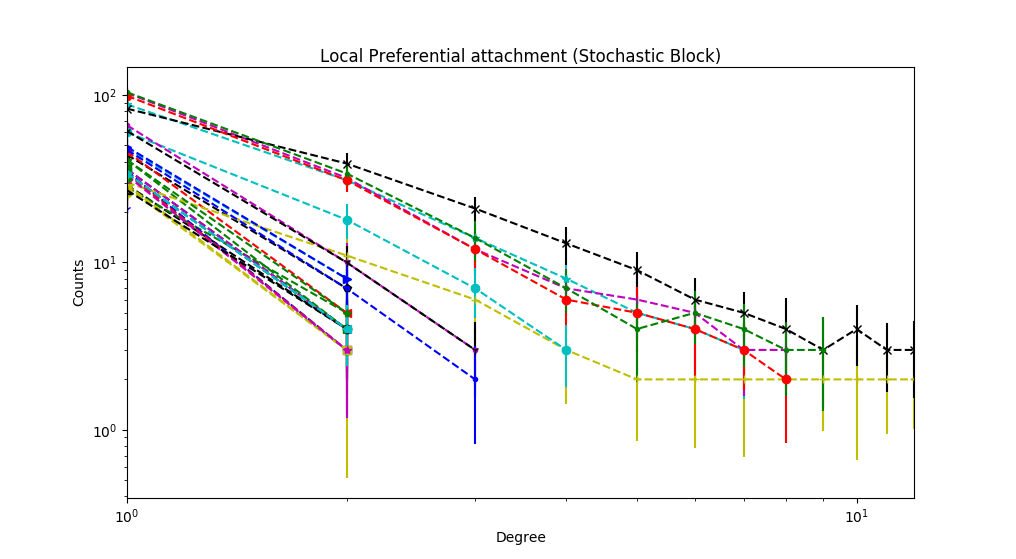
\includegraphics[scale=0.27]{img/expe/2_mmsb/figure_2} 
	\endminipage
	\minipage{0.27\textwidth}
	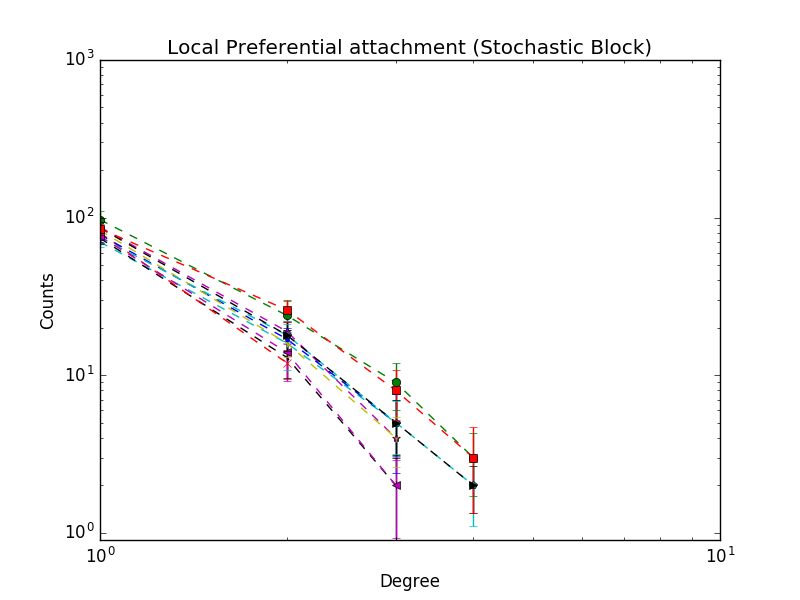
\includegraphics[scale=0.27]{img/expe/3_mmsb/figure_2}
	\endminipage
		\vspace{-0.28cm}
	\minipage{0.27\textwidth}
	\includegraphics[scale=0.27]{img/expe/1_mmsb/figure_3}
	\endminipage
	\minipage{0.27\textwidth}
	\includegraphics[scale=0.27]{img/expe/2_mmsb/figure_3} 
	\endminipage
	\minipage{0.27\textwidth}
	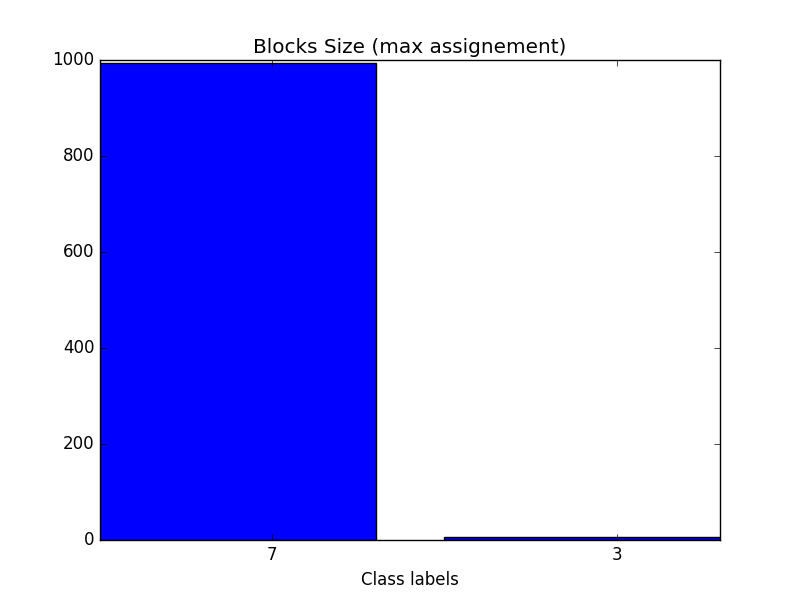
\includegraphics[scale=0.27]{img/expe/3_mmsb/figure_3}
	\endminipage

    \vspace{0.2cm}
	 ILFM

	\minipage{0.27\textwidth}
	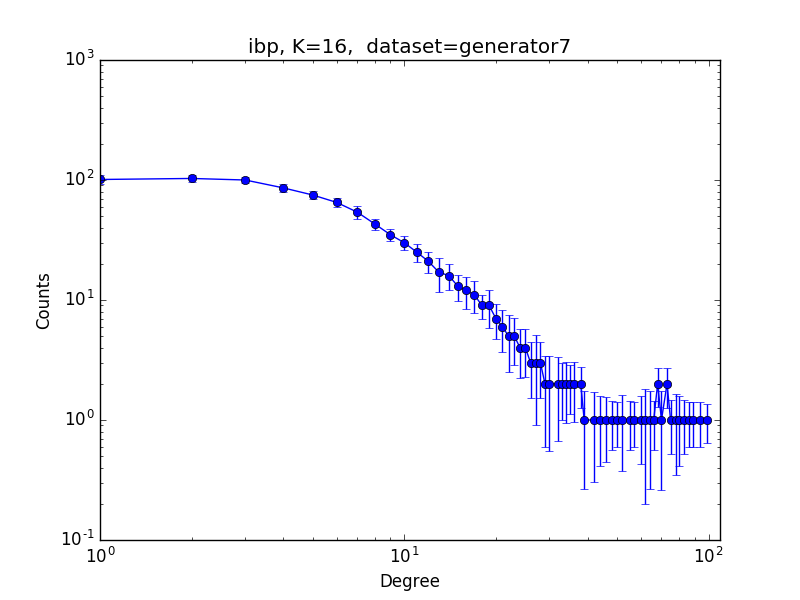
\includegraphics[scale=0.27]{img/expe/1_ibp/figure_1}
	\endminipage
		\minipage{0.27\textwidth}
	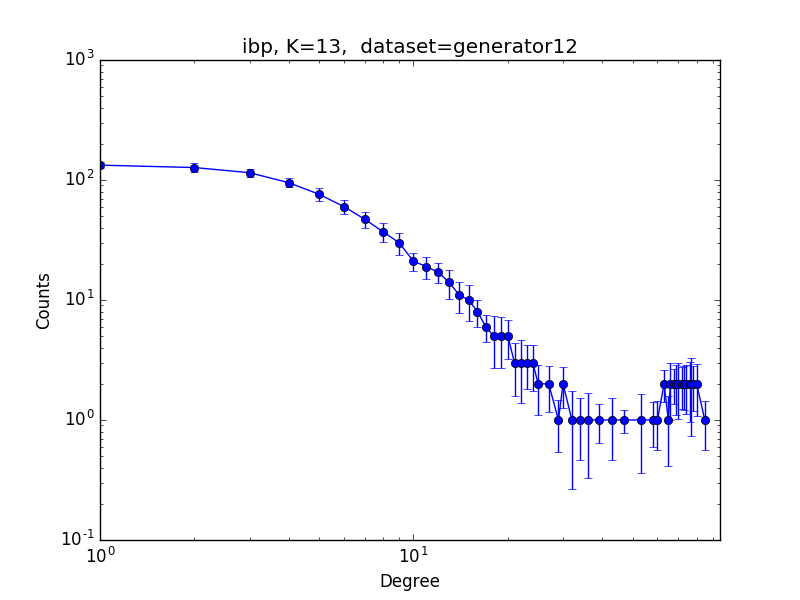
\includegraphics[scale=0.27]{img/expe/2_ibp/figure_1}
	\endminipage
	\minipage{0.27\textwidth}
	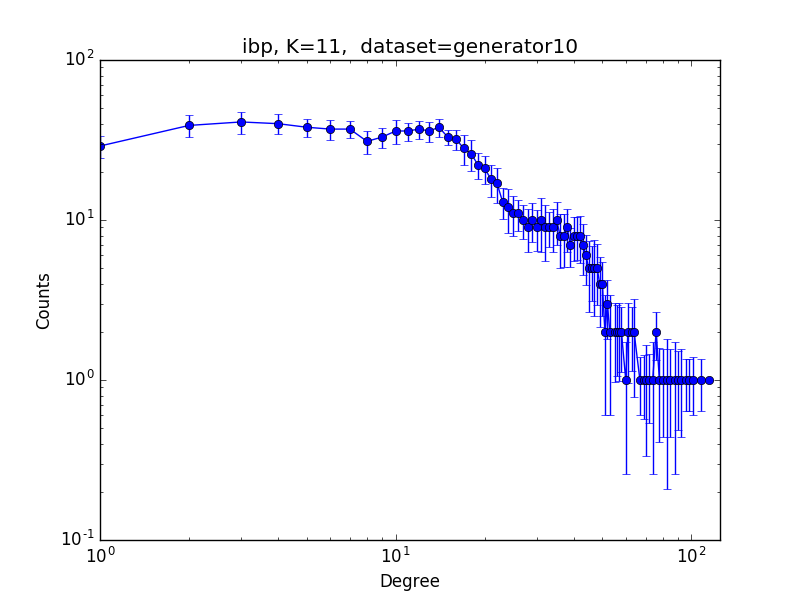
\includegraphics[scale=0.27]{img/expe/3_ibp/figure_1}
	\endminipage
		\vspace{-0.29cm}
	\minipage{0.27\textwidth}
	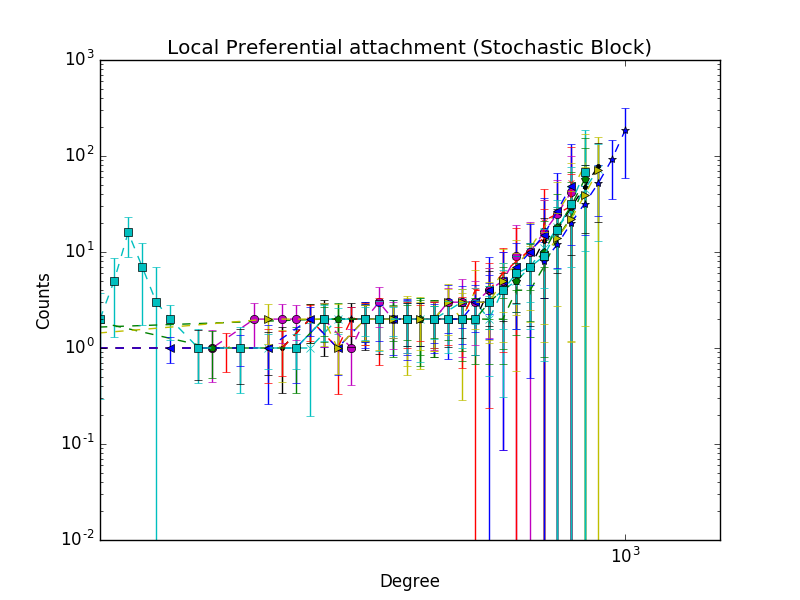
\includegraphics[scale=0.27]{img/expe/1_ibp/figure_2}
	\endminipage
		\minipage{0.27\textwidth}
	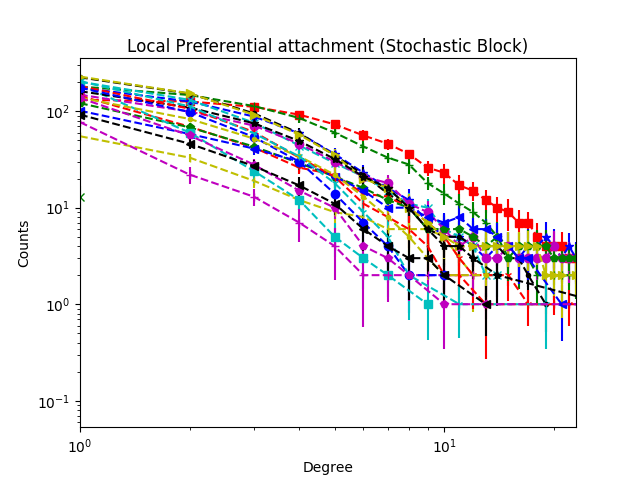
\includegraphics[scale=0.27]{img/expe/2_ibp/figure_2} 
	\endminipage
	\minipage{0.27\textwidth}
	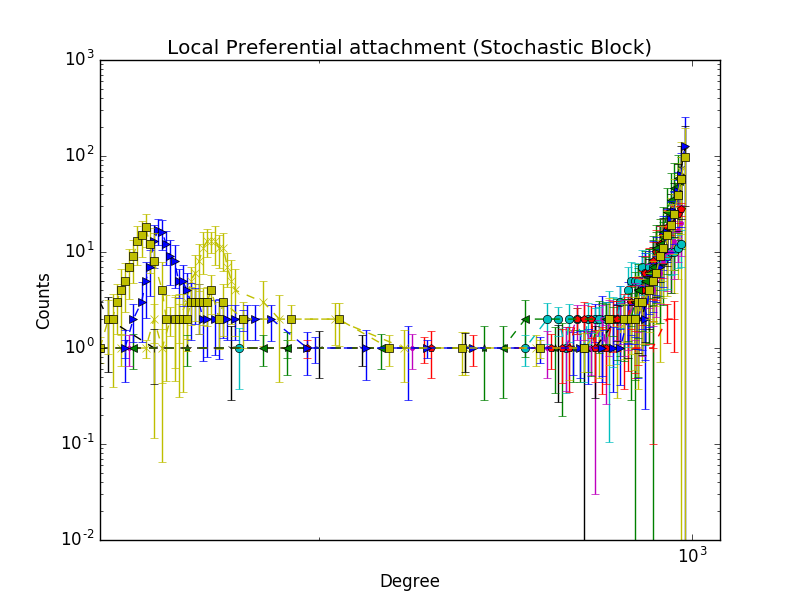
\includegraphics[scale=0.27]{img/expe/3_ibp/figure_2}
	\endminipage
		\vspace{-0.28cm}
	\minipage{0.27\textwidth}
	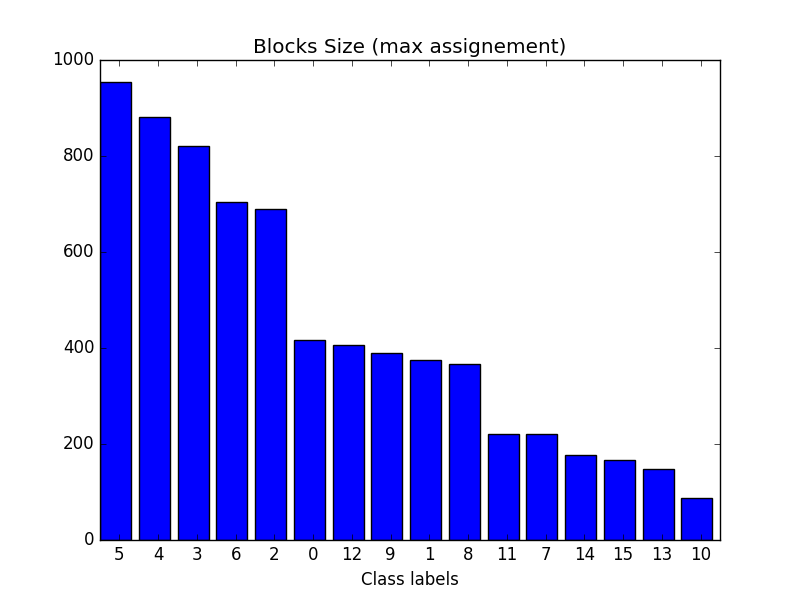
\includegraphics[scale=0.27]{img/expe/1_ibp/figure_3}
	\endminipage
	\minipage{0.27\textwidth}
	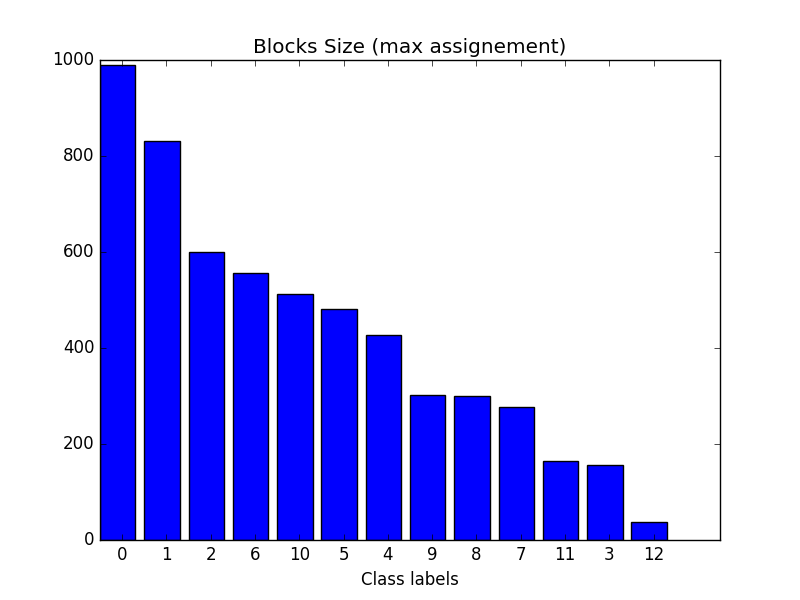
\includegraphics[scale=0.27]{img/expe/2_ibp/figure_3} 
	\endminipage
	\minipage{0.27\textwidth}
	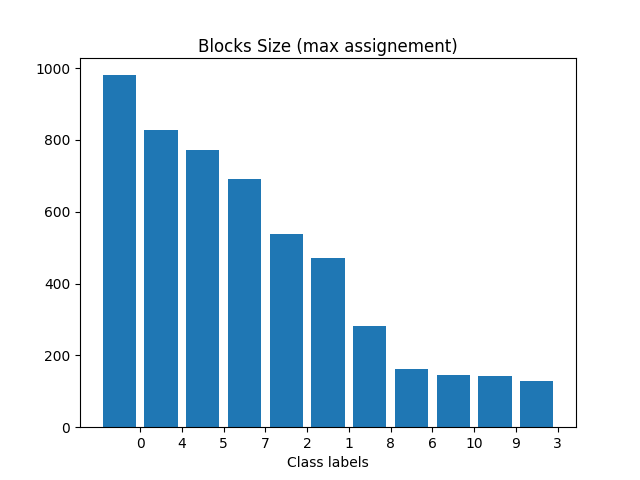
\includegraphics[scale=0.27]{img/expe/3_ibp/figure_3}
	\endminipage
    \caption{Network 1,2 and 3}

\end{figure}

\begin{figure}[ht]
    \vspace{-3cm}
	\centering IMMSB\\
	\minipage{0.27\textwidth}
	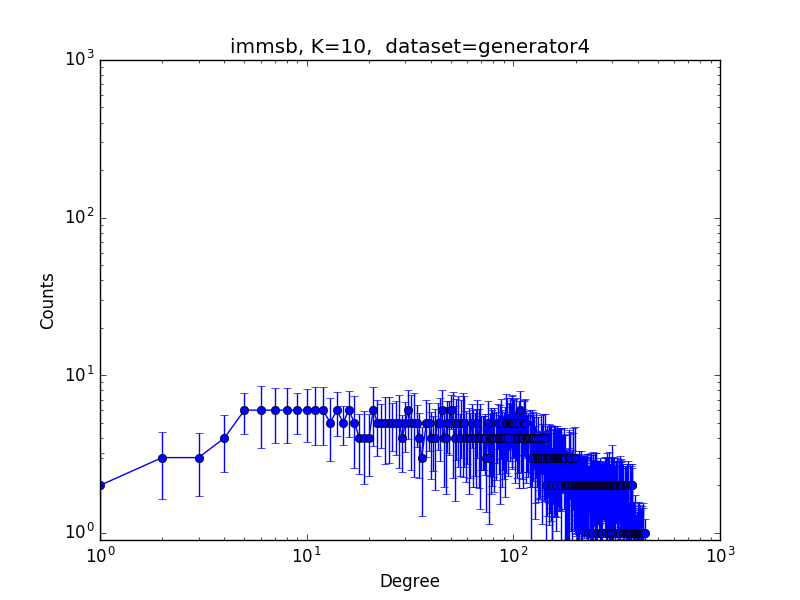
\includegraphics[scale=0.27]{img/expe/4_mmsb/figure_1}
	\endminipage
		\minipage{0.27\textwidth}
	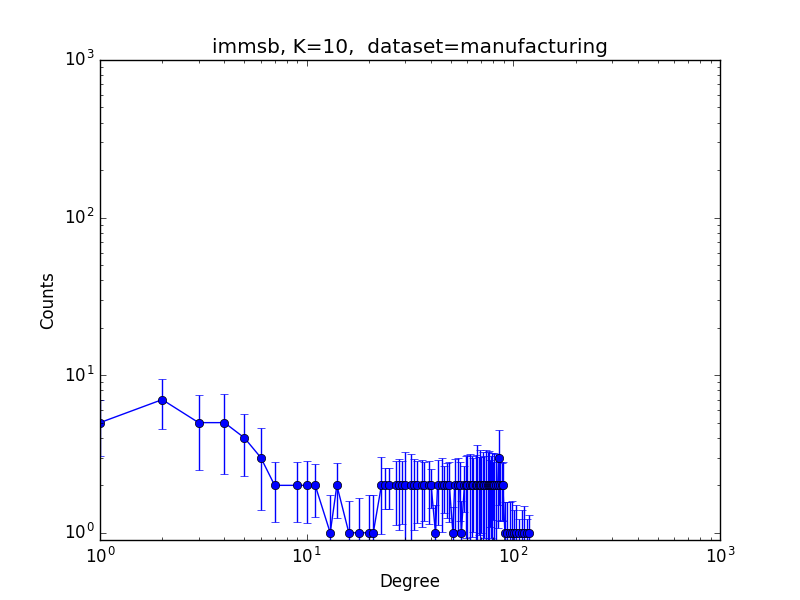
\includegraphics[scale=0.27]{img/expe/5_mmsb/figure_1}
	\endminipage
	\minipage{0.27\textwidth}
	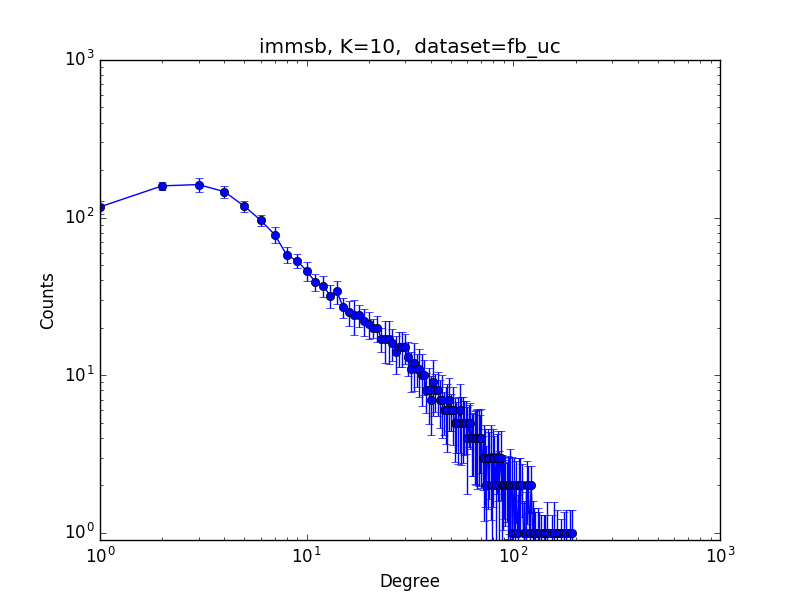
\includegraphics[scale=0.27]{img/expe/6_mmsb/figure_1}
	\endminipage
		\vspace{-0.29cm}
	\minipage{0.27\textwidth}
	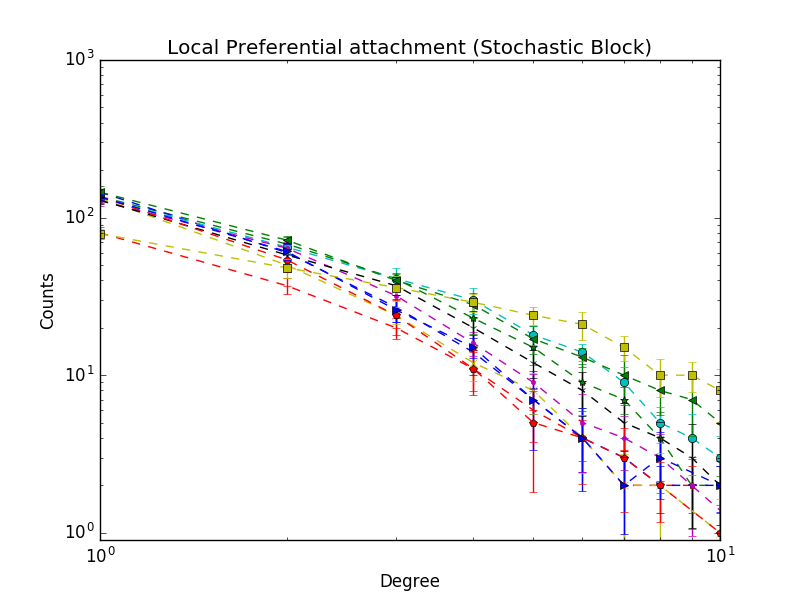
\includegraphics[scale=0.27]{img/expe/4_mmsb/figure_2}
	\endminipage
		\minipage{0.27\textwidth}
	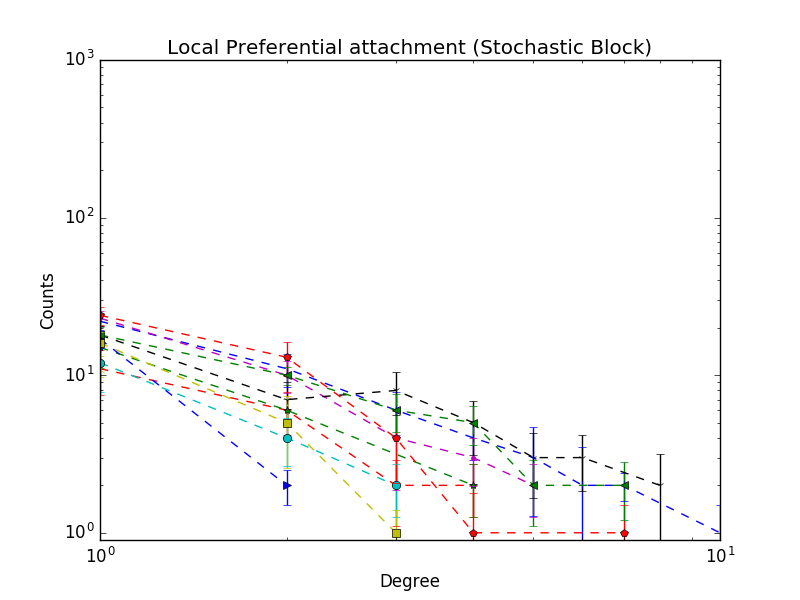
\includegraphics[scale=0.27]{img/expe/5_mmsb/figure_2} 
	\endminipage
	\minipage{0.27\textwidth}
	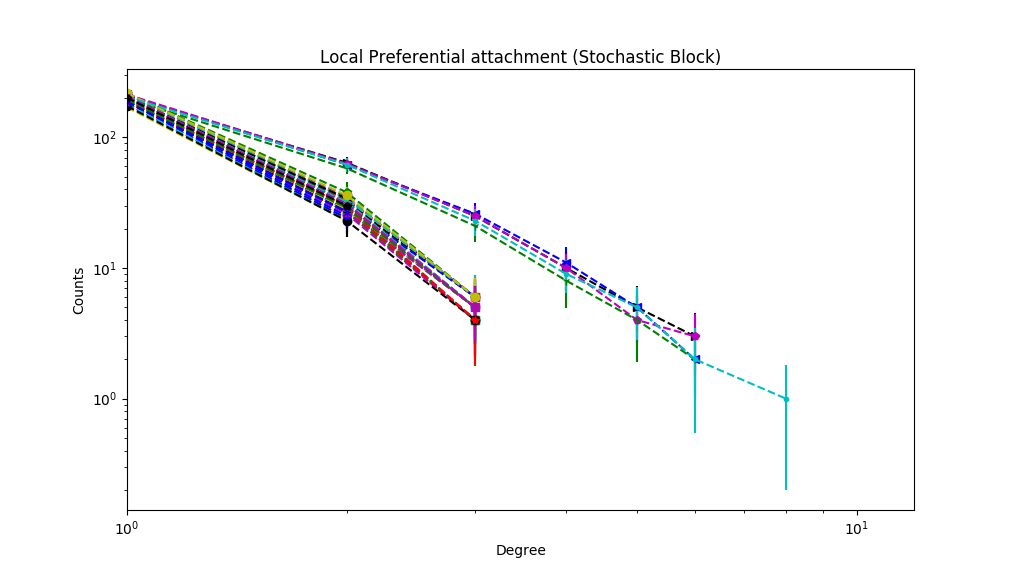
\includegraphics[scale=0.27]{img/expe/6_mmsb/figure_2}
	\endminipage
		\vspace{-0.28cm}
	\minipage{0.27\textwidth}
	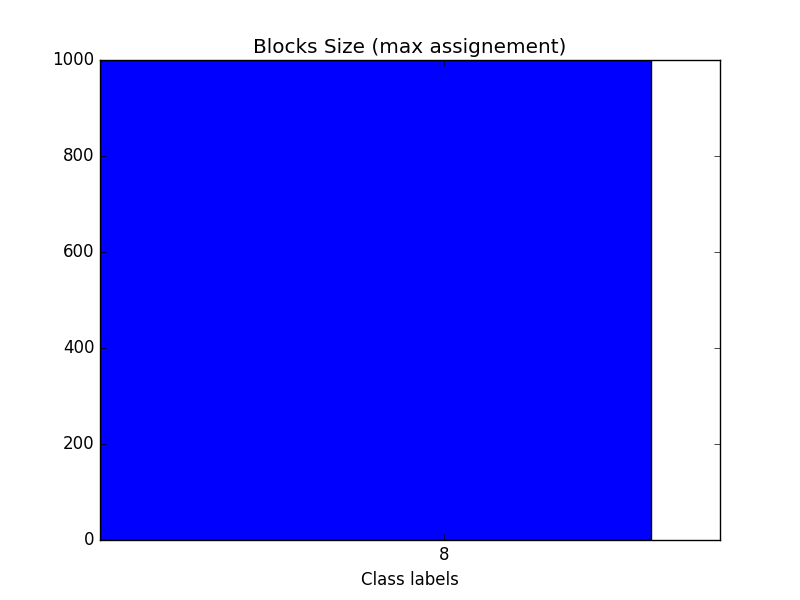
\includegraphics[scale=0.27]{img/expe/4_mmsb/figure_3}
	\endminipage
	\minipage{0.27\textwidth}
	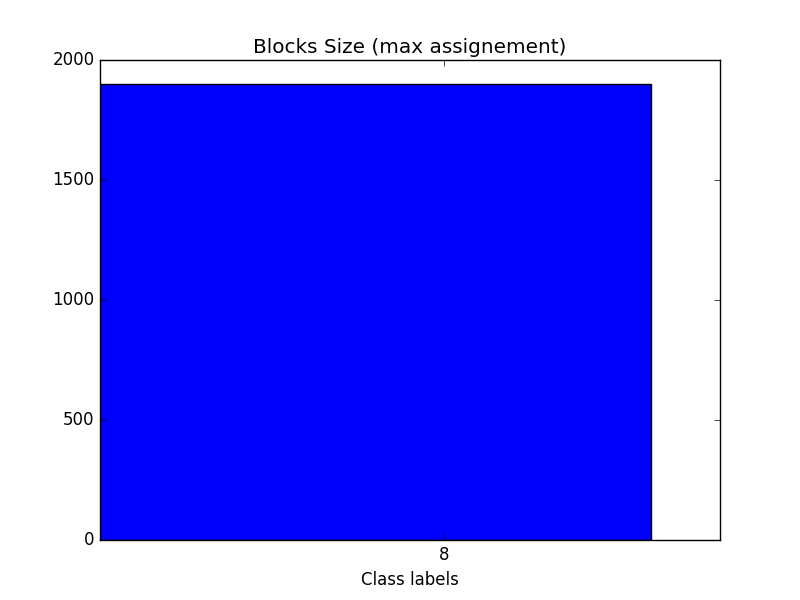
\includegraphics[scale=0.27]{img/expe/6_mmsb/figure_3} 
	\endminipage
	\minipage{0.27\textwidth}
	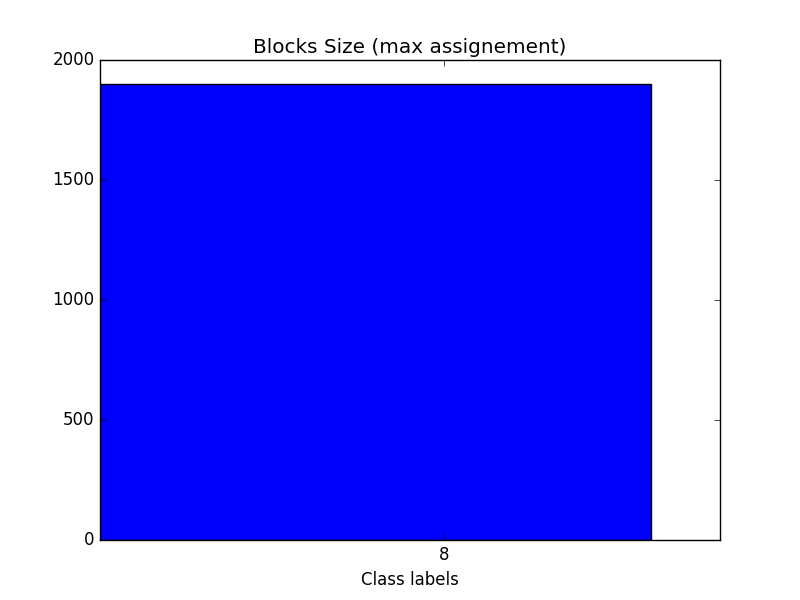
\includegraphics[scale=0.27]{img/expe/6_mmsb/figure_3}
	\endminipage

    \vspace{0.2cm}
	 ILFM

	\minipage{0.27\textwidth}
	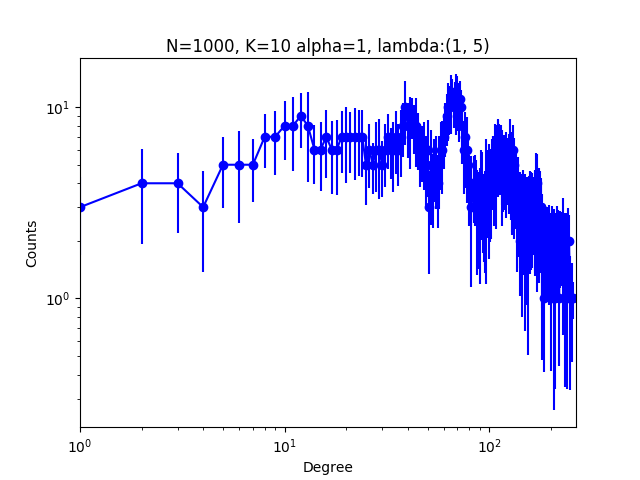
\includegraphics[scale=0.27]{img/expe/4_ibp/figure_1}
	\endminipage
		\minipage{0.27\textwidth}
	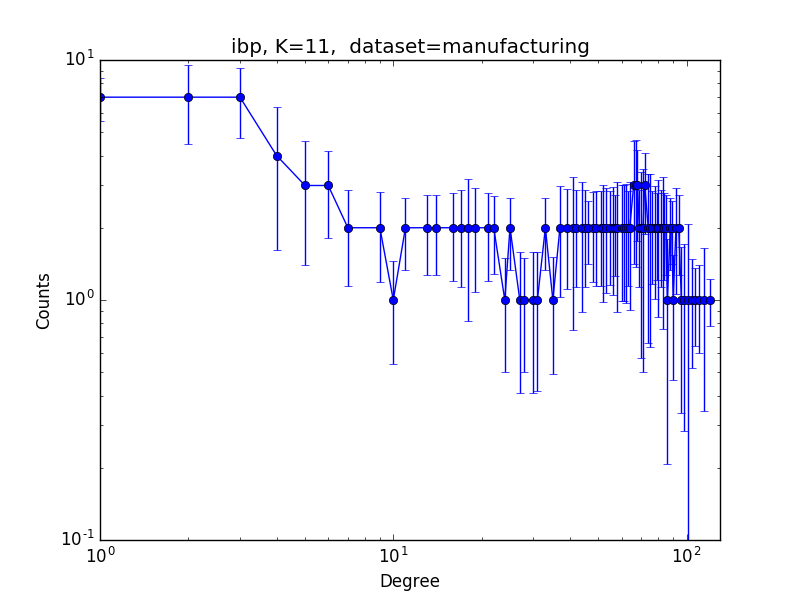
\includegraphics[scale=0.27]{img/expe/5_ibp/figure_1}
	\endminipage
	\minipage{0.27\textwidth}
	
\includegraphics[scale=0.27]{img/expe/6_ibp/figure_1}
	\endminipage
		\vspace{-0.29cm}
	\minipage{0.27\textwidth}
	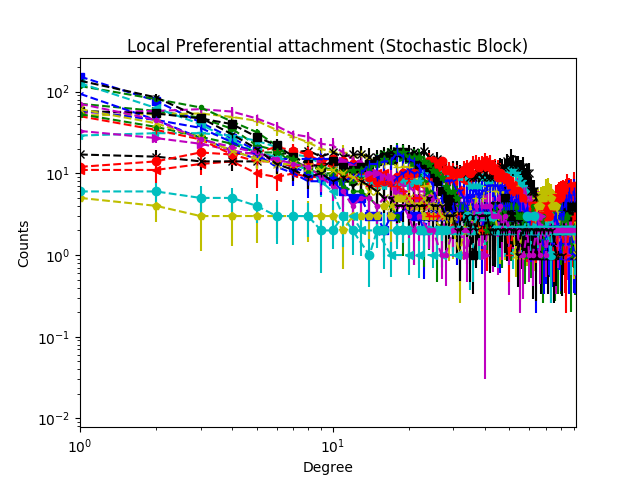
\includegraphics[scale=0.27]{img/expe/4_ibp/figure_2}
	\endminipage
		\minipage{0.27\textwidth}
	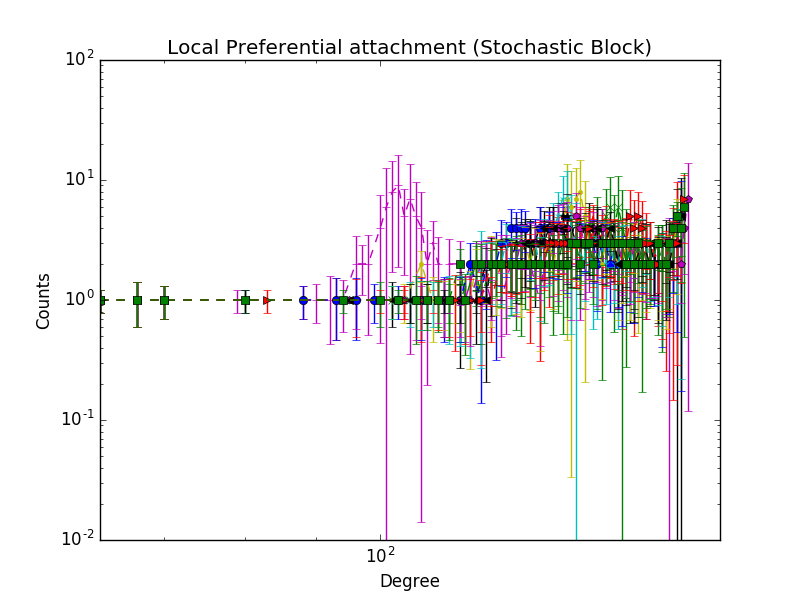
\includegraphics[scale=0.27]{img/expe/5_ibp/figure_2} 
	\endminipage
	\minipage{0.27\textwidth}
	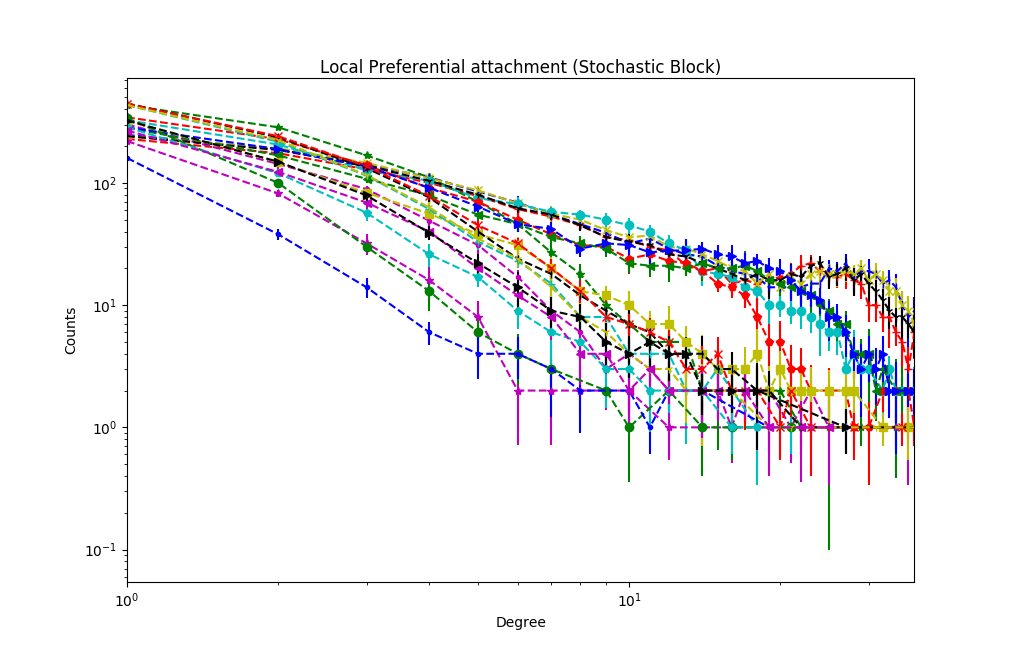
\includegraphics[scale=0.27]{img/expe/6_ibp/figure_2}
	\endminipage
		\vspace{-0.28cm}
	\minipage{0.27\textwidth}
	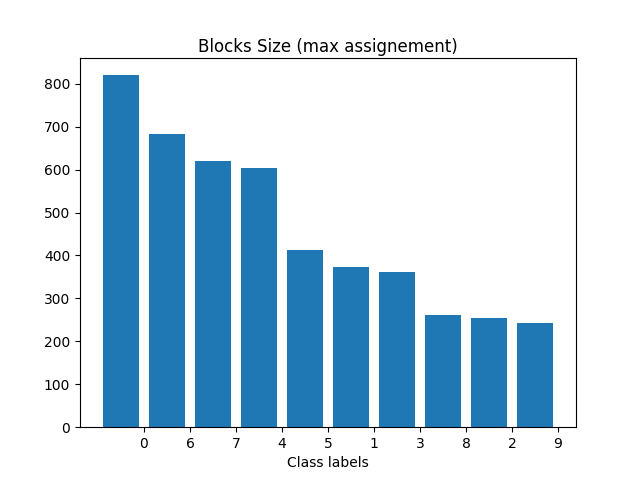
\includegraphics[scale=0.27]{img/expe/4_ibp/figure_3}
	\endminipage
	\minipage{0.27\textwidth}
	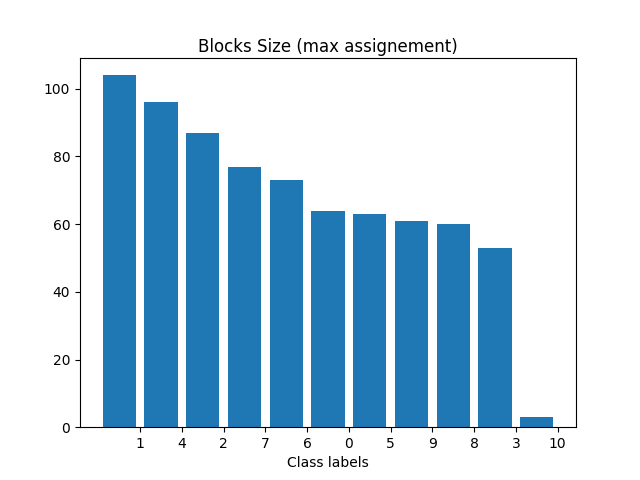
\includegraphics[scale=0.27]{img/expe/5_ibp/figure_3} 
	\endminipage
	\minipage{0.27\textwidth}
	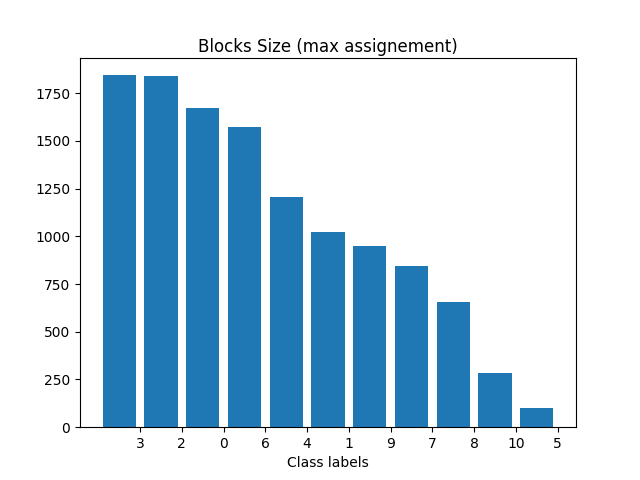
\includegraphics[scale=0.27]{img/expe/6_ibp/figure_3}
	\endminipage
    \caption{Network 4, manufacturing and Facebook}

\end{figure}


\clearpage

\subsection{Homophily}

\clearpage
\section{$M_g$}

\subsection{Burstiness}


\begin{figure}[ht]
    \vspace{-3cm}
	\centering IMMSB\\
	\minipage{0.27\textwidth}
	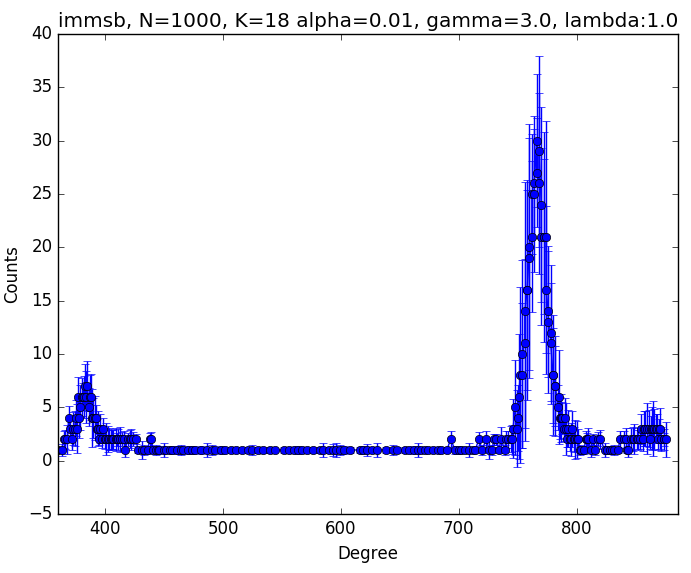
\includegraphics[scale=0.27]{img/M_g_peaks/figure_1}
	\endminipage
		\minipage{0.27\textwidth}
	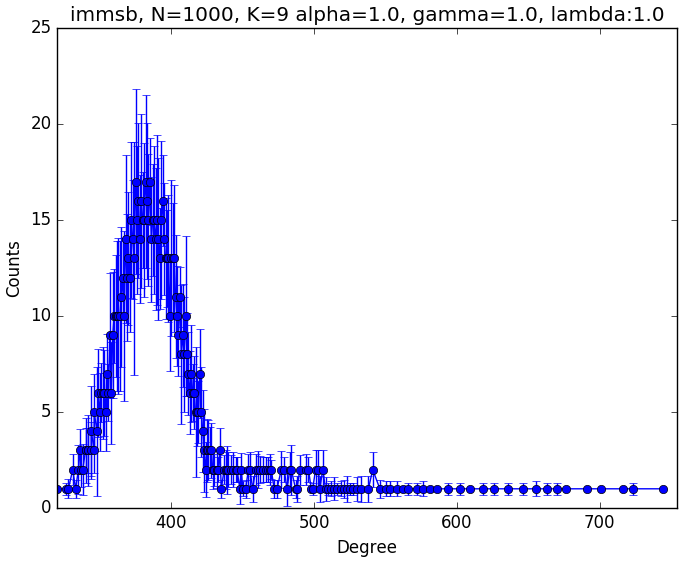
\includegraphics[scale=0.27]{img/M_g_power_law/figure_1}
	\endminipage
	\minipage{0.27\textwidth}
	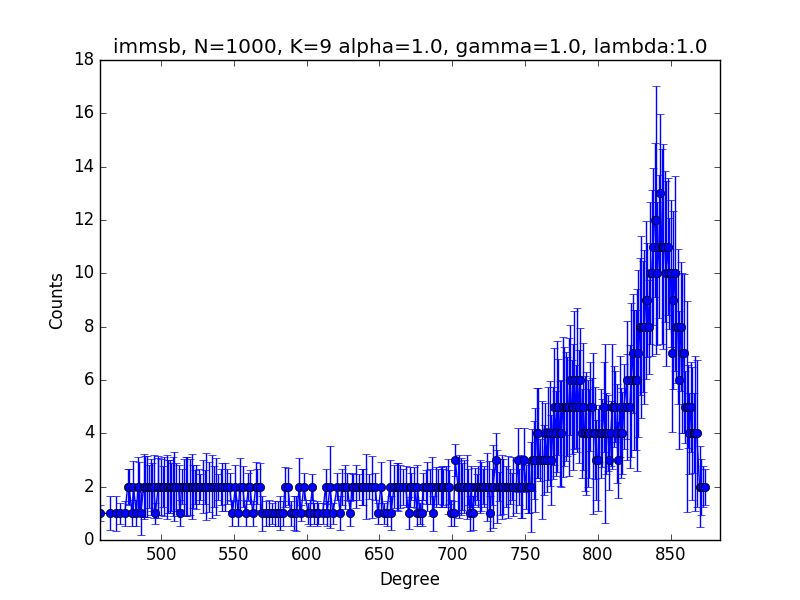
\includegraphics[scale=0.27]{img/M_g_regular/figure_1}
	\endminipage
		\vspace{-0.29cm}
	\minipage{0.27\textwidth}
	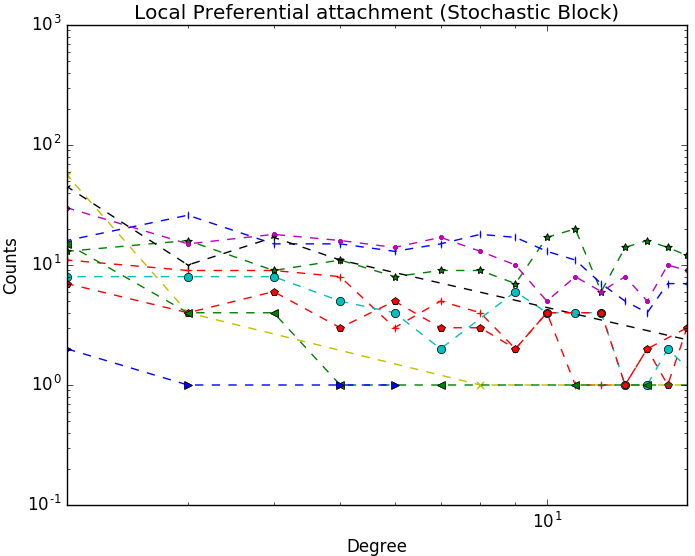
\includegraphics[scale=0.27]{img/M_g_peaks/figure_3}
	\endminipage
		\minipage{0.27\textwidth}
	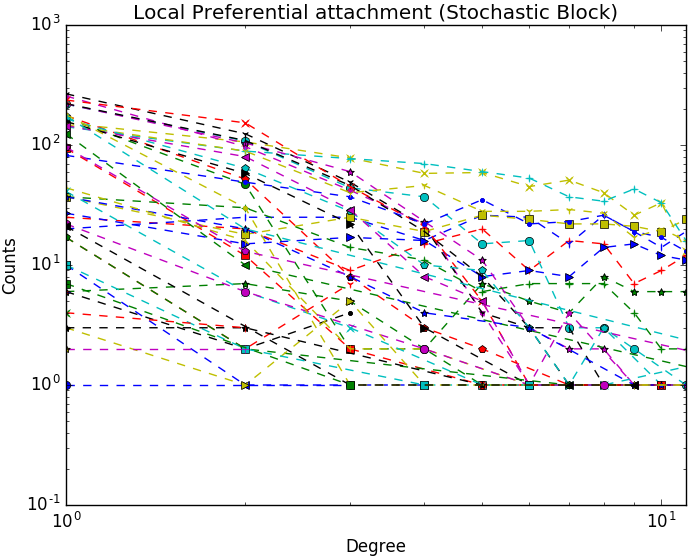
\includegraphics[scale=0.27]{img/M_g_power_law/figure_3} 
	\endminipage
	\minipage{0.27\textwidth}
	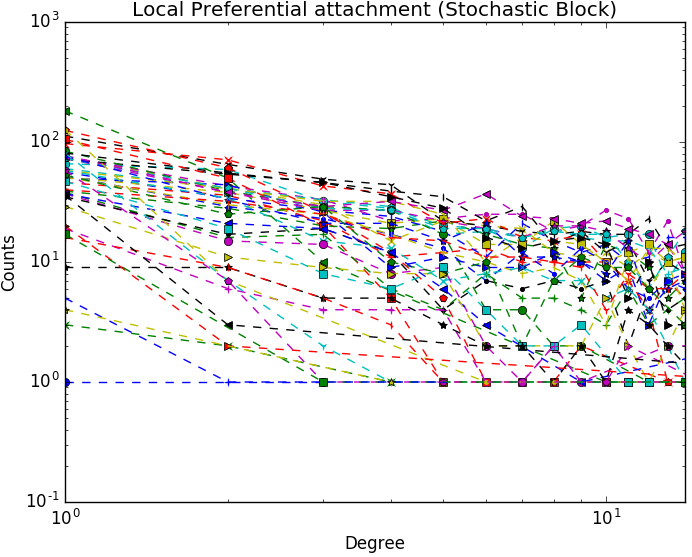
\includegraphics[scale=0.27]{img/M_g_regular/figure_3}
	\endminipage
		\vspace{-0.28cm}
	\minipage{0.27\textwidth}
	\includegraphics[scale=0.27]{img/M_g_peaks/figure_5}
	\endminipage
	\minipage{0.27\textwidth}
	\includegraphics[scale=0.27]{img/M_g_power_law/figure_5} 
	\endminipage
	\minipage{0.27\textwidth}
	\includegraphics[scale=0.27]{img/M_g_regular/figure_5}
	\endminipage

    \vspace{0.2cm}
	 ILFM

	\minipage{0.27\textwidth}
	\includegraphics[scale=0.27]{img/ilfm/1/figure_1}
	\endminipage
		\minipage{0.27\textwidth}
	\includegraphics[scale=0.27]{img/ilfm/2/figure_1}
	\endminipage
	\minipage{0.27\textwidth}
	\includegraphics[scale=0.27]{img/ilfm/3/figure_1}
	\endminipage
		\vspace{-0.29cm}
	\minipage{0.27\textwidth}
	\includegraphics[scale=0.27]{img/ilfm/1/figure_3}
	\endminipage
		\minipage{0.27\textwidth}
	\includegraphics[scale=0.27]{img/ilfm/2/figure_3} 
	\endminipage
	\minipage{0.27\textwidth}
	\includegraphics[scale=0.27]{img/ilfm/3/figure_3}
	\endminipage
		\vspace{-0.28cm}
	\minipage{0.27\textwidth}
	\includegraphics[scale=0.27]{img/ilfm/1/figure_5}
	\endminipage
	\minipage{0.27\textwidth}
	\includegraphics[scale=0.27]{img/ilfm/2/figure_5} 
	\endminipage
	\minipage{0.27\textwidth}
	\includegraphics[scale=0.27]{img/ilfm/3/figure_5}
	\endminipage
    \caption{\tiny{Generated Networks with IMMSB (top) and ILFM (bottom) for three different settings (same set than for figure \ref{fig:gen_blocks_mmsb}). The top rows measure the global preferential attachment through the overall degree distribution. The middle row measure the local preferential attachment through the local degree distribution. The last row measure the feature burstiness through the block membership distribution.}}
	\label{fig:gen_burst}
\end{figure}

\clearpage

\subsection{Homophily}


\end{document}
